% Created with jtex v.0.1.10
\documentclass{article}
\PassOptionsToPackage{short, nodayofweek}{datetime}


% Start Curvenote Definitions

% Pass Options Section
% base
\PassOptionsToPackage{normalem}{ulem}
\PassOptionsToPackage{utf8}{inputenc}

% template
\PassOptionsToPackage{framemethod=TikZ}{mdframed}
\PassOptionsToPackage{x11names, svgnames}{xcolor}

%%% PACKAGES

% base
\usepackage{inputenc}
\usepackage{url}
\usepackage{graphicx}
\usepackage{adjustbox}
\usepackage{amssymb}
\usepackage{amsfonts}
\usepackage{amsmath}
\usepackage{enumitem}
\usepackage{nicefrac}
\usepackage{booktabs}
\usepackage{microtype}
\usepackage{hyperref}
\usepackage{ulem}
\usepackage{enumitem}
\usepackage{float}
\usepackage{datetime}
\usepackage{xkeyval}
\usepackage{framed}
\usepackage{doi}

% template
\usepackage{natbib}
\usepackage{fancyvrb}
\usepackage{mdframed}
\usepackage{xcolor}

%%%


%%%% Setup Section

% base
\graphicspath{{.}}
% template
\sloppy
\newenvironment{aside}{\begin{framed}}{\end{framed}}
\newmdenv[linewidth=2pt,linecolor=CornflowerBlue,topline=false,bottomline=false,rightline=false,leftline=true,skipabove=20,skipbelow=20,leftmargin=20,rightmargin=20]{callout}
\newfloat{code}{thp}{loc}
\floatname{code}{Program}
\raggedbottom
\bibliographystyle{abbrvnat}
\setcitestyle{authoryear,open={(},close={)},semicolon,aysep={,}}

% End Curvenote Definitions


%%%%%%%%%%%%%%%%%%%%%%%%%%%%%%%%%%%%%%%%%%%%%%%%%%
%%%%%%%%%%%%%%%%%  math commands  %%%%%%%%%%%%%%%%
\newcommand{\q}{\koppa}
\newcommand{\Ex}{\mathbb{E}}
%%%%%%%%%%%%%%%%%%%%%%%%%%%%%%%%%%%%%%%%%%%%%%%%%%

% colors for hyperlinks
\hypersetup{colorlinks=true, allcolors=blue}
\hypersetup{
pdftitle={\@title},
pdfsubject={},
pdfauthor={\@author},
pdfkeywords={},
addtopdfcreator={Written in Curvenote}
}

\usepackage{curvenote}

\title{}

\newdate{articleDate}{28}{3}{2023}
\date{\displaydate{articleDate}}

\author{}

\begin{document}

\maketitle
\keywords{}/SequentialEGM

document

\subsection{Multivariate Interpolation on Non-Rectilinear Grids}\label{sec:gpr}

This section presents alternative interpolation methods for non-rectilinear grids. First, I present the relatively simple case of fast warped interpolation on a curvilinear grid, which improves upon the interpolation in \citet{White2015}. Then, I present a machine learning approach to interpolation on unstructured grids based on Gaussian Process Regression as presented in \citet{Scheidegger2019}.

\subsubsection{Warped Grid Interpolation (WGI)}\label{Warped Grid Interpolation (WGI)}

Assume we have a set of points indexed by $(i,j)$ in two-dimensional space for which we have corresponding functional values in a third dimension, such that $f(x_{ij},y_{ij}) = z_{ij}$. In practice, we are interested in cases where the $z_{ij}$ are difficult to compute and $f(x_{ij},y_{ij})$ is unknown, so we are unable to compute them at other values of $x$ and $y$ --- which is why we want to interpolate\footnote{For this illustration, we generate $z$'s arbitrarily using the function

\begin{equation}
f(x,y) = (xy)^{1/4}.
\end{equation}}. These $(x_{ij},y_{ij})$ points however are not evenly spaced and do not form a rectilinear grid which would make it easy to interpolate the function off the grid. Nevertheless, these points do have a regular structure as we will see.

\begin{figure}[!htbp]
\centering
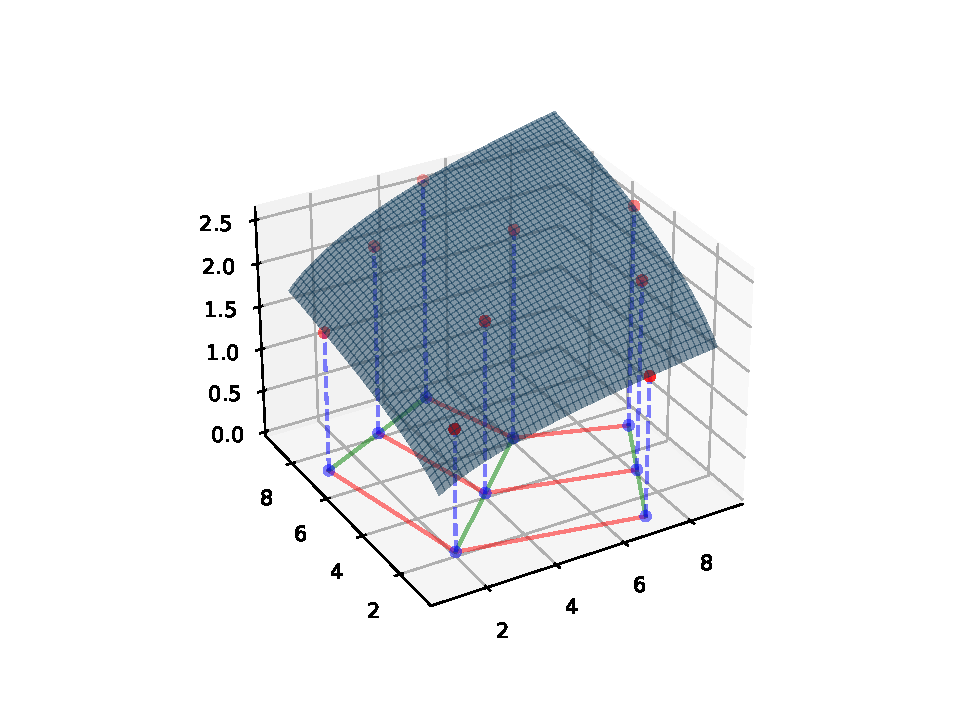
\includegraphics[width=0.7\linewidth]{Figures/WarpedInterpolation.pdf}
\caption{True function and curvilinear grid of points for which we know the value of the function.}
\label{fig:warped_interp}
\end{figure}

In Figure~Figure~\ref{fig:warped_interp}, we can see the true function in three-dimensional space, along with the points for which we actually know the value of the function. The underlying regular structure comes from the points' position in the matrix, the $(i,j)$ coordinates. If we join the points along every row and every column, we can see that the resulting grid is regular and piecewise affine (curvilinear).

In Figure~Figure~\ref{fig:homotopy} we see the values of the function at their index coordinate points in the matrix. We can see that there exists a mapping between the curvilinear grid and the index coordinates of the matrix.

\begin{figure}[!htbp]
\centering
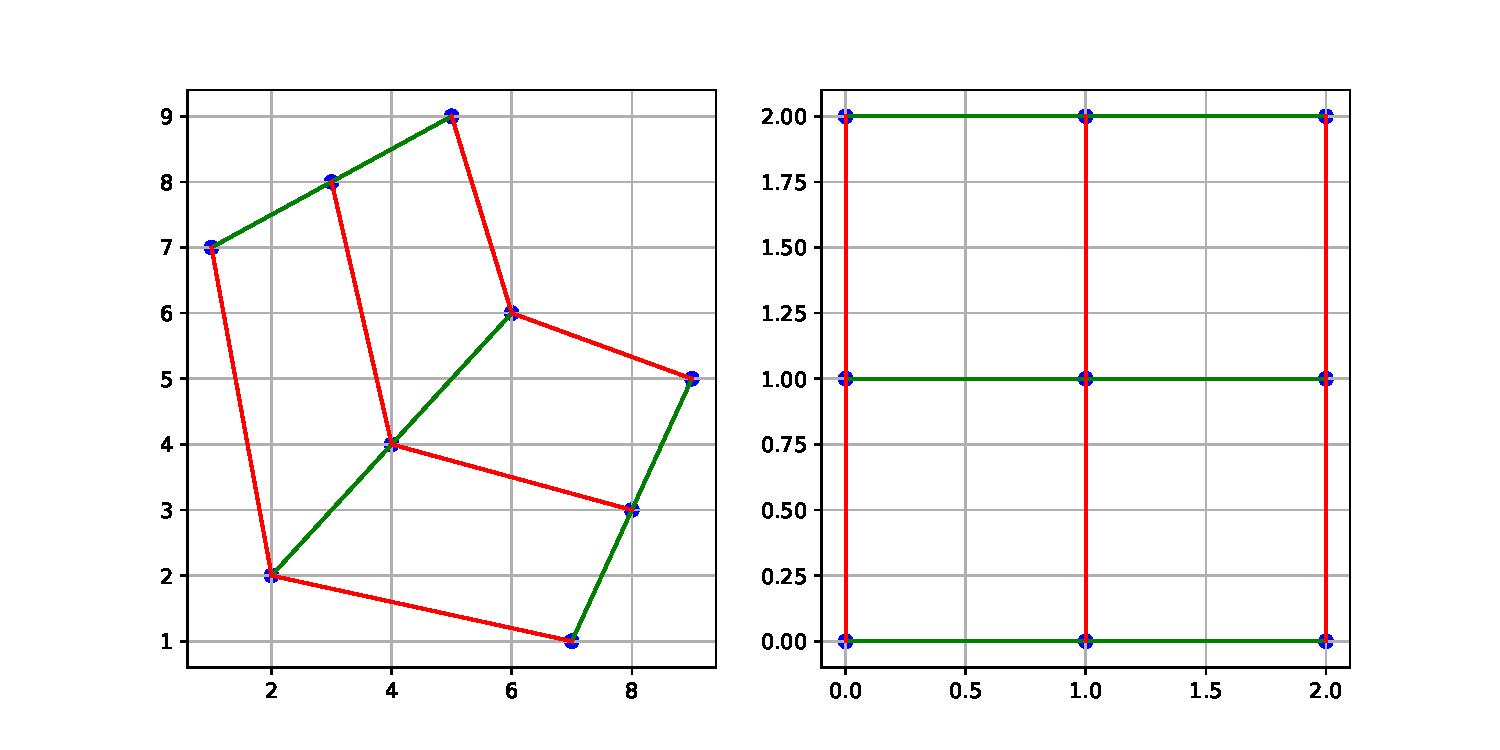
\includegraphics[width=0.7\linewidth]{Figures/Homotopy.pdf}
\caption{Homotopy between the curvilinear grid and the index coordinates of the matrix.}
\label{fig:homotopy}
\end{figure}

The objective is to be able to interpolate the value of the function at any point off the grid, where presumably we are only interested in points internal to the curvilinear space and not outside the boundaries. For example, we can imagine that we want an approximation to the function at the point $(x,y) = (3, 5)$ pictured Figure~Figure~\ref{fig:mapping}. If we could find the corresponding point in the coordinate grid, interpolation would be straightforward. We can find where the $x$-coordinate of the point of interest intersects with the index-coordinates of the matrix. This is similar to assuming that we have 3 linear interpolators formed by connecting the points on the green lines in the x-direction, and for each interpolator we can approximate the corresponding y and z values using the grid data. Now, for each circle in Figure~Figure~\ref{fig:mapping}, we have a corresponding pair $(y,z)$, and we can interpolate in the y-direction to find the corresponding z-value for the point's y-coordinate\footnote{For more examples of the Warped Grid Interpolation method in action, see the github project \href{https://github.com/alanlujan91/multinterp/blob/main/notebooks/CurvilinearInterpolation.ipynb}{\texttt{}}.}.

\begin{figure}[!htbp]
\centering
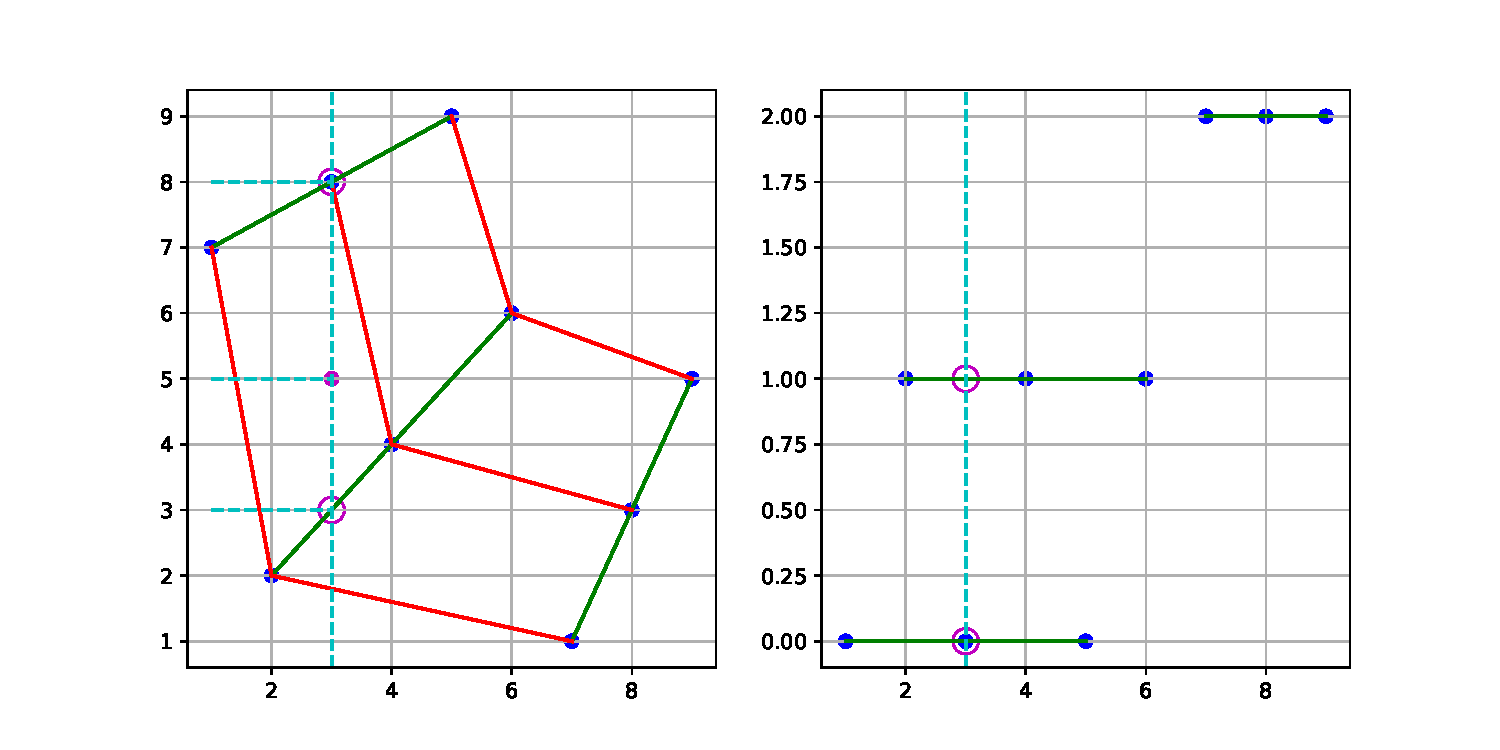
\includegraphics[width=0.7\linewidth]{Figures/Mapping.pdf}
\caption{The method consist of extending the loci of points in the $x$ dimension to find the corresponding crossing points in the $y$ dimension.}
\label{fig:mapping}
\end{figure}

\subsubsection{Unstructured Grids}\label{Unstructured Grids}

Unstructured interpolation arises in many dynamic programming applications when using the Endogenous Grid Method because the first-order conditions might be highly non-linear and non-monotonic, or because boundary constraints induce kinks in the policy and value functions. In these cases, the grid points generated by the EGM step are not evenly spaced, leading to the need for curvilinear interpolation. We saw in the previous subsection an approach to curvilinear interpolation based on \citet{White2015} that is incapable of interpolation on structured grids. A similar approach was presented in \citet{Ludwig2018} which used Delaunay interpolation. However, this approach is not well suited for our purposes because triangulation can be computationally intensive and slow, often offsetting the efficiency gains from the Endogenous Grid Method.

As an alternative to these methods, I introduce the use of Gaussian Process Regression (GPR) along with the Endogenous Grid Method. GPR is computationally efficient, and tools exist to easily parallelize and take advantage of hardware such as Graphics Processing Units (GPU)\footnote{\citet{Gardner2018}}.

\paragraph{Gaussian Process Regression}\label{Gaussian Process Regression}

A Gaussian Process is an infinite dimensional random process for which every subset of random variables is jointly Gaussian or has a multivariate normal distribution.

\begin{equation}
\begin{gathered}
    \mathbf{X} \sim \mathcal{N}(\mathbf{\mu}, \mathbf{\Sigma}) \quad \text{s.t.} \quad x_i \sim \mathcal{N}(\mu_i, \sigma_{ii}) \\
    \text{and} \quad  \sigma_{ij} = \Ex[(x_i - \mu_i)(x_j - \mu_j)] \quad \forall i,j \in \{1, \ldots, n\}.
  \end{gathered}
\end{equation}

where

\begin{equation}
\mathbf{X} = \begin{bmatrix}
    x_1    \\
    x_2    \\
    \vdots \\
    x_n
  \end{bmatrix}
  \quad
  \mathbf{\mu} = \begin{bmatrix}
    \mu_1  \\
    \mu_2  \\
    \vdots \\
    \mu_n
  \end{bmatrix}
  \quad
  \mathbf{\Sigma} = \begin{bmatrix}
    \sigma_{11} & \sigma_{12} & \cdots & \sigma_{1n} \\
    \sigma_{21} & \sigma_{22} & \cdots & \sigma_{2n} \\
    \vdots      & \vdots      & \ddots & \vdots      \\
    \sigma_{n1} & \sigma_{n2} & \cdots & \sigma_{nn}
  \end{bmatrix}.
\end{equation}

Being infinitely dimensional, a Gaussian Process can be used to represent a probability distribution over the space of functions in $n$ dimensions. Thus, a Gaussian Process Regression is used to find the best fit function to a set of data points.

\begin{equation}
\mathbb{P}(\mathbf{f} | \mathbf{X}) = \mathcal{N}(\mathbf{f} | \mathbf{m}, \mathbf{K})
\end{equation}

where $\mathbf{f}$ is the vector of function values at the points $\mathbf{X}$, $\mathbf{m}$ is the mean of the function, and $\mathbf{K}$ is a kernel function that describes the covariance between the function values at different points.

A standard kernel function is the squared exponential kernel, or the radial basis function kernel, which is defined as

\begin{equation}
k(\mathbf{x}_i, \mathbf{x}_j) = \sigma^2_f \exp\left(-\frac{1}{2l^2} (\mathbf{x}_i - \mathbf{x}_j)' (\mathbf{x}_i - \mathbf{x}_j)\right).
\end{equation}

Using GPR to interpolate a function $f$, we can both predict the value of the function at a point $\mathbf{x}_*$ and the uncertainty in the prediction, which provides useful information as to the accuracy of the approximation.

\paragraph{An example of the GPR}\label{An example of the GPR}

In Figure~Figure~\ref{fig:true_function}, we see the function we are trying to approximate along with a sample of data points for which we know the value of the function. In practice, the value of the function is unknown and/or expensive to compute, so we must use a limited amount of data to approximate it.

\begin{figure}[!htbp]
\centering
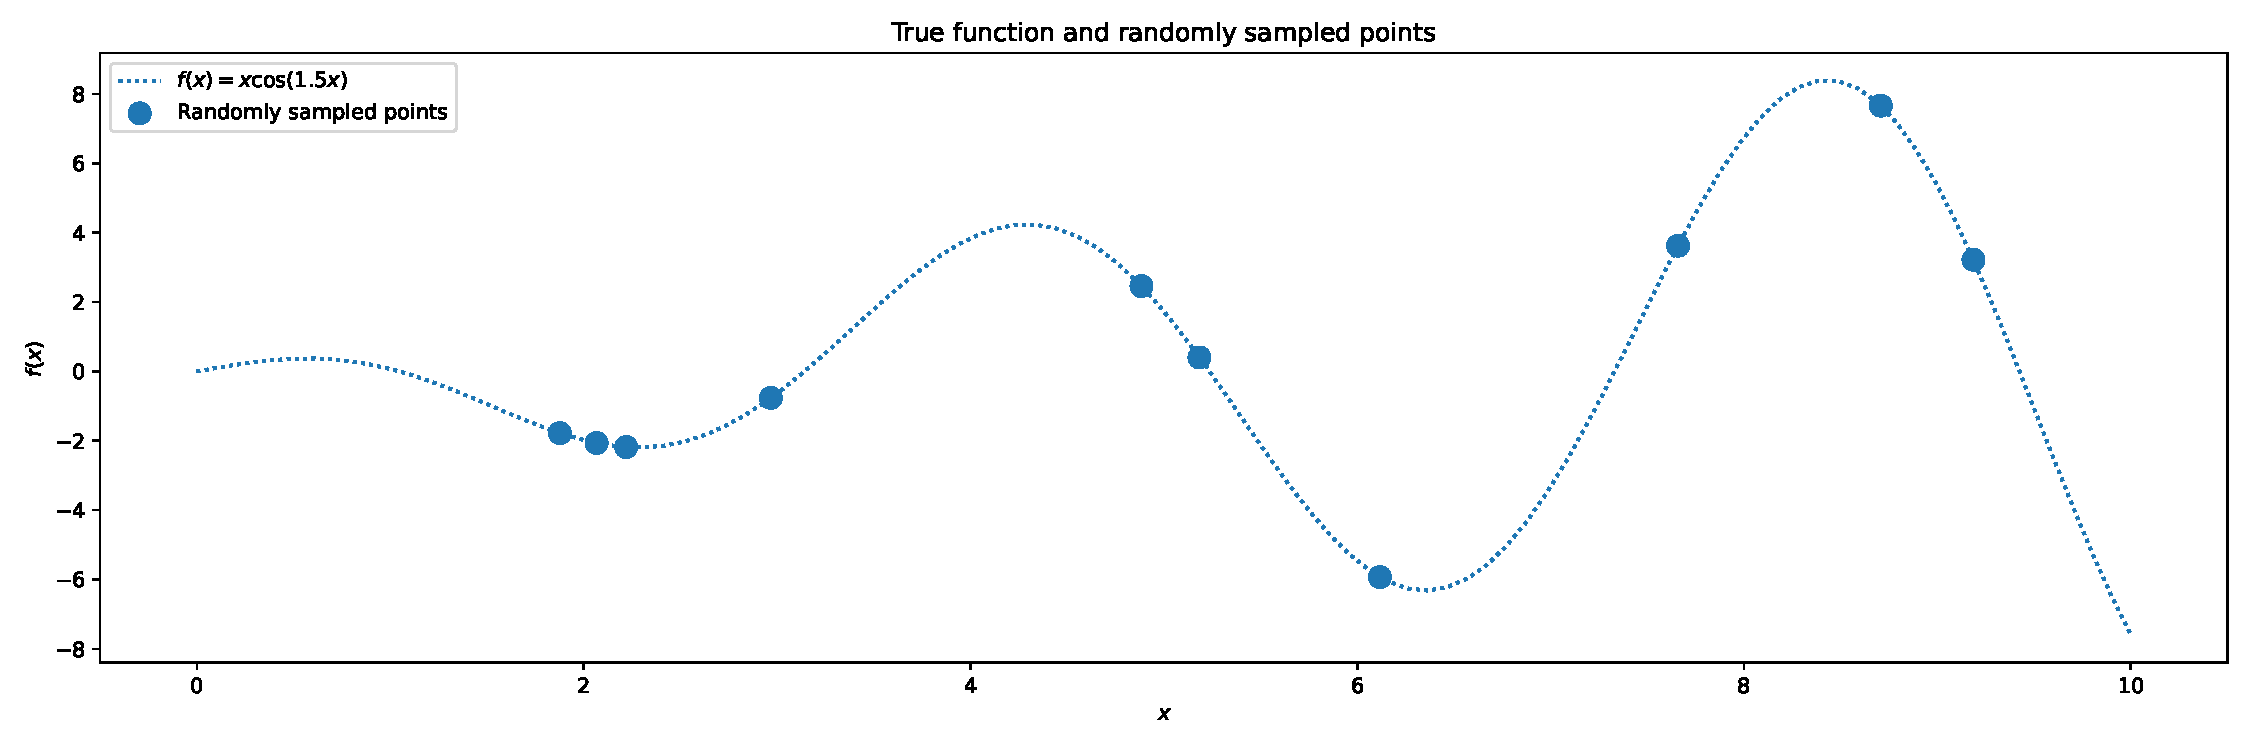
\includegraphics[width=0.7\linewidth]{Figures/true_function.pdf}
\caption{The true function that we are trying to approximate and a sample of data points.}
\label{fig:true_function}
\end{figure}

As we discussed, a Gaussian Process is an infinite dimensional random process which can be used to represent a probability of distributions over the space of functions. In Figure~Figure~\ref{fig:gpr_sample}, we see a random sample of functions from the GPR posterior, which is a Gaussian Process conditioned on fitting the data. From this small sample of functions, we can see that the GP generates functions that fit the data well, and the goal of GPR is to find the one function that best fits the data given some hyperparameters by minimizing the negative log-likelihood of the data.

\begin{figure}[!htbp]
\centering
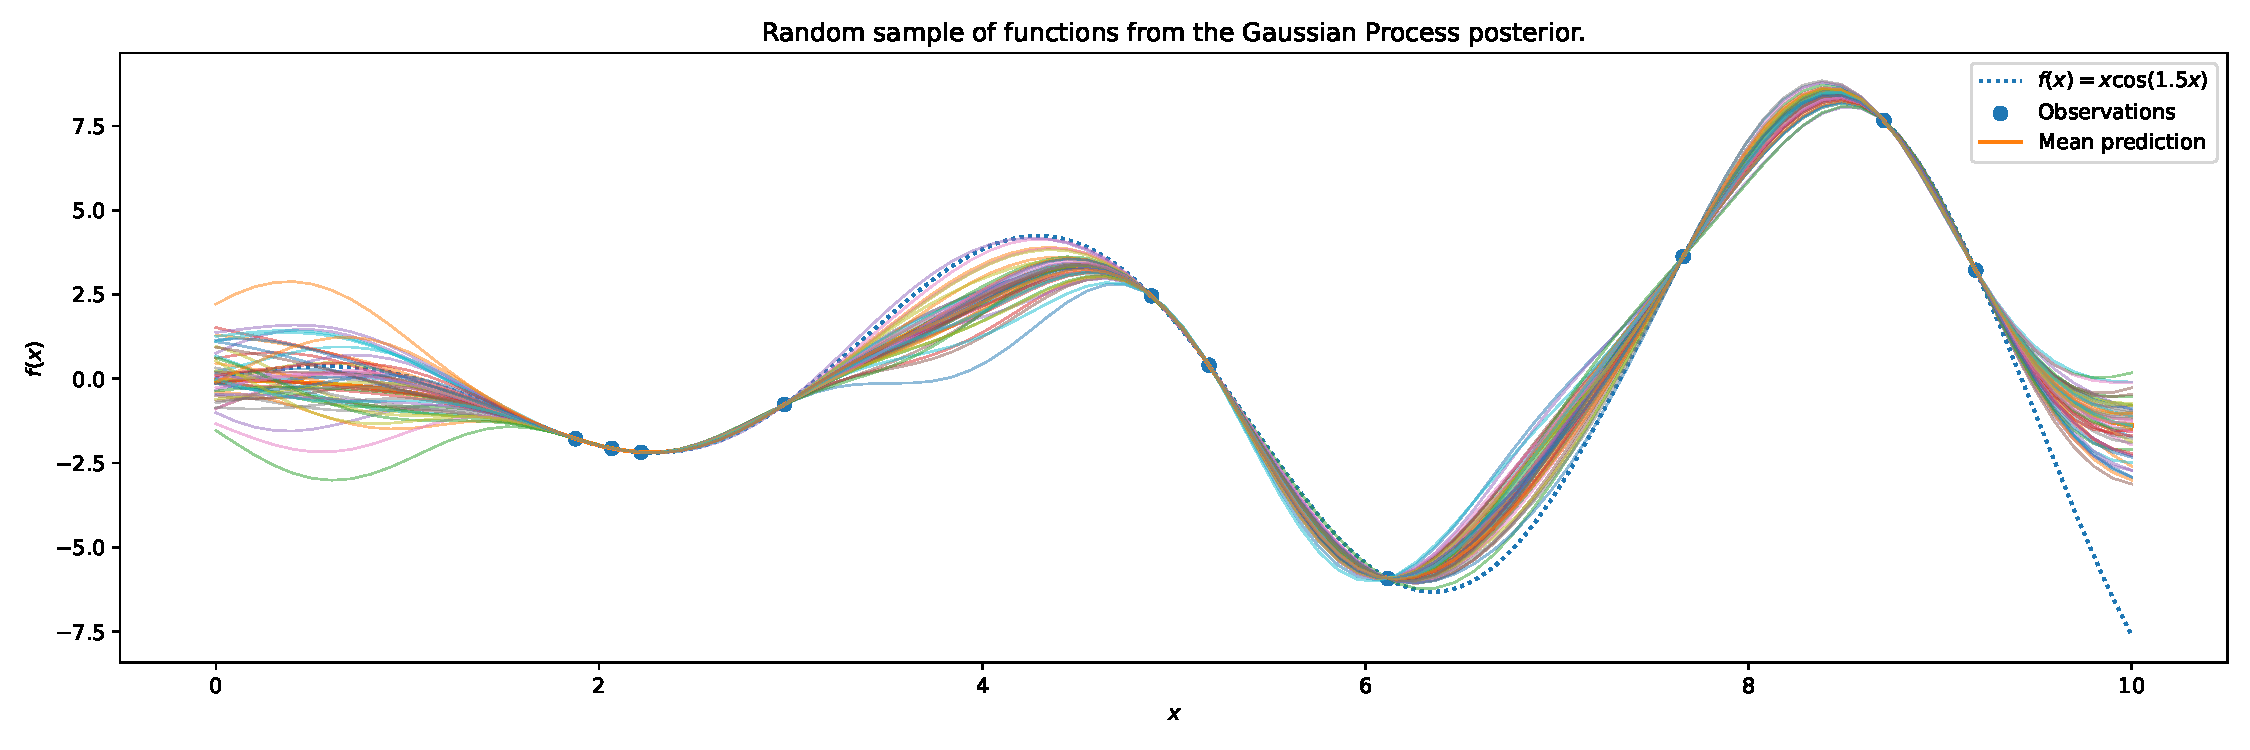
\includegraphics[width=0.7\linewidth]{Figures/gpr_sample.pdf}
\caption{A random sample of functions from the GPR posterior that fit the data. The goal of GPR is to find the function that best fits the data.}
\label{fig:gpr_sample}
\end{figure}

In Figure~Figure~\ref{fig:gpr}, we see the result of GPR with a particular parametrization\footnote{For details see notebook.} of the kernel function. The dotted line shows the true function, while the blue dots show the known data points. GPR provides the mean function which best fits the data, represented in the figure as an orange line. The shaded region represents a 95\% confidence interval, which is the uncertainty of the predicted function. Along with finding the best fit of the function, GPR provides the uncertainty of the prediction, which is useful information as to the accuracy of the approximation.

\begin{figure}[!htbp]
\centering
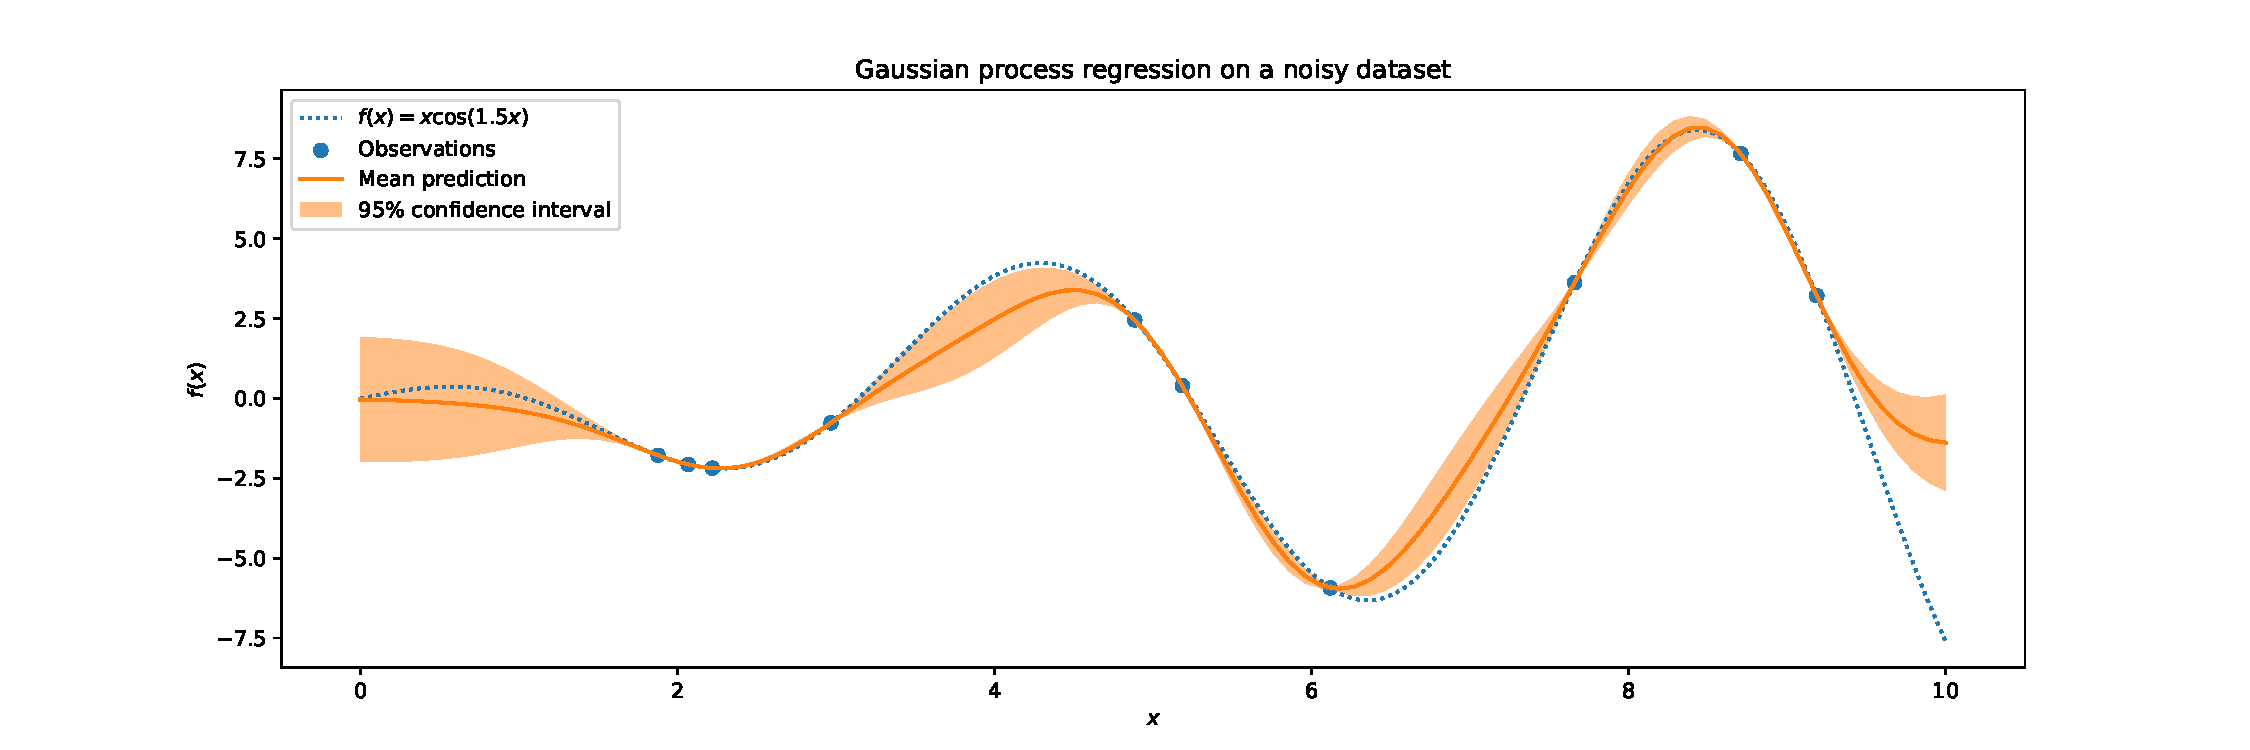
\includegraphics[width=0.7\linewidth]{Figures/gpr.pdf}
\caption{GPR finds the function that best fits the data given some hyperparameters. GPR then optimizes over the parameter space to find the function that minimizes the negative log-likelihood of the data.}
\label{fig:gpr}
\end{figure}

Web

[figure]list=no

[table]list=no

document

\clearpage
\bibliography{main.bib}

\end{document}
